%% LaTeX Beamer presentation template (requires beamer package)
%% see http://latex-beamer.sourceforge.net/
%% idea contributed by H. Turgut Uyar
%% template based on a template by Till Tantau
%% this template is still evolving - it might differ in future releases!

\PassOptionsToPackage{subsection=false}{beamerouterthememiniframes}
\documentclass{beamer}

\mode<presentation>
{
%\useoutertheme[subsection=false]{miniframes}
\usetheme{Berlin}
\setbeamertemplate{navigation symbols}{} 
\setbeamercovered{dynamic}
\setbeamertemplate{footline}{}
}

\hypersetup{pdfstartview={FitH}}

\usepackage[brazil]{babel}
\usepackage[utf8]{inputenc}
%\usepackage{lmodern}
\usepackage{mathptmx}% font definitions, try \usepackage{ae} instead of the following
\usepackage[scaled=.90]{helvet}% three lines if you don't like this look
\usepackage{courier}
\usepackage[T1]{fontenc}
\usepackage{url}
\usepackage{graphicx}
\usepackage{array}
\usepackage{colortbl}
\usepackage{tikz}
\usepackage{pgfplots}
\usepackage{colortbl}
\usepackage{xcolor}
\usepackage{pgf-pie}
\pgfplotsset{compat=1.7}

\definecolor{n_red}{HTML}{D7191C}
\definecolor{n_orange}{HTML}{FD9B61}
\definecolor{n_green}{HTML}{3F745A}
\definecolor{n_green_bg}{HTML}{AAE6C9}
\definecolor{n_blue}{HTML}{2B83BA}
\definecolor{n_violet}{HTML}{AC146D}
\definecolor{n_yellow}{HTML}{D2D221}
\definecolor{RawSienna}{cmyk}{0,0.72,1,0.45}
\definecolor{olive}{rgb}{0.3, 0.4, .1}

\newenvironment{colorblock}[3]{%
  \setbeamercolor{block body}{#2}
  \setbeamercolor{block title}{#3}
  \begin{block}{#1}}{\end{block}}

\newcommand{\colorize}[2]{\textbf{\textcolor{#1}{#2}}}

  
\title{Um Algoritmo de Escalonamento para Redução do Consumo de
    Energia em Computação em Nuvem}

%\subtitle{}

% - Use the \inst{?} command only if the authors have different
%   affiliation.
%\author{F.~Author\inst{1} \and S.~Another\inst{2}}
\author[shortname]{Pedro Paulo Vezzá Campos}
\institute[shortinst]{
	MAC\oldstylenums{0499} -- Trabalho de Formatura Supervisionado \\
	Instituto de Matemática e Estatística \\
		Universidade de São Paulo, São Paulo, Brasil \\
	\url{pedro@vezza.com.br}
	}

\date{\today}


% This is only inserted into the PDF information catalog. Can be left
% out.
\subject{Um Algoritmo de Escalonamento para Redução do Consumo de
    Energia em Computação em Nuvem}



% If you have a file called "university-logo-filename.xxx", where xxx
% is a graphic format that can be processed by latex or pdflatex,
% resp., then you can add a logo as follows:

% \pgfdeclareimage[height=0.5cm]{university-logo}{university-logo-filename}
% \logo{\pgfuseimage{university-logo}}



% Delete this, if you do not want the table of contents to pop up at
% the beginning of each subsection:
\AtBeginSection[]
{
\begin{frame}<beamer>
\frametitle{Agenda}
\tableofcontents[currentsection,currentsubsection]
\end{frame}
}

% If you wish to uncover everything in a step-wise fashion, uncomment
% the following command:

\beamerdefaultoverlayspecification{<+->}


\begin{document}


\begin{frame}
\titlepage
\end{frame}

\begin{frame}
\frametitle{Agenda}
\begin{colorblock}{Motivação \& Conceitos}{bg=n_violet!5}{bg=n_violet!100}
	\begin{itemize}
		\item Consumo energético
		\item Escalonamento de fluxos de trabalho
		\item Um algoritmo clássico: \emph{Heterogeneous Earliest Finish Time}
	\end{itemize}
\end{colorblock}

\begin{colorblock}{Experimentos}{bg=n_violet!5}{bg=n_violet!100}
	\begin{itemize}
		\item O desenvolvimento de um novo algoritmo: Êxitos e frustrações
	\end{itemize}
\end{colorblock}

\begin{colorblock}{Conclusões}{bg=n_violet!5}{bg=n_violet!100}
	\begin{itemize}
		\item Análise das contribuições e resultados obtidos
	\end{itemize}
\end{colorblock}
%\tableofcontents
% You might wish to add the option [pausesections]
\end{frame}


%%%%%%%%%%%%%%%%%%%%%%%%%%%%%%%%%%%%%%%%%%%%%%%%%%%%%%%%%%%%%%%%%%%%%%%%%%%%%%%%
%%%%%%%%%%%%%%%%%%%%%%%%%%%%%%%%%%%%%%%%%%%%%%%%%%%%%%%%%%%%%%%%%%%%%%%%%%%%%%%%
\section{Motivação}
\subsection{}

%%%%%%%%%%%%%%%%%%%%%%%%%%%%%%%%%%%%%%%%%%%%%%%%%%%%%%%%%%%%%%%%%%%%%%%%%%%%%%%%
%\begin{frame}
%\frametitle{Motivação}
%\begin{itemize}
%	\item A \colorize{n_red}{Lei de Moore} está chegando ao fim da sua vida
%	\item Novas tendências: \colorize{n_green}{computação verde}, eficiência
%	energética
%	\item \colorize{n_violet}{Computação em nuvem}: Racionalização e
%	compartilhamento de recursos
%\end{itemize}
%
%\end{frame}

%%%%%%%%%%%%%%%%%%%%%%%%%%%%%%%%%%%%%%%%%%%%%%%%%%%%%%%%%%%%%%%%%%%%%%%%%%%%%%%%
\begin{frame}
\frametitle{}

\begin{figure}[htp]
\begin{center}
  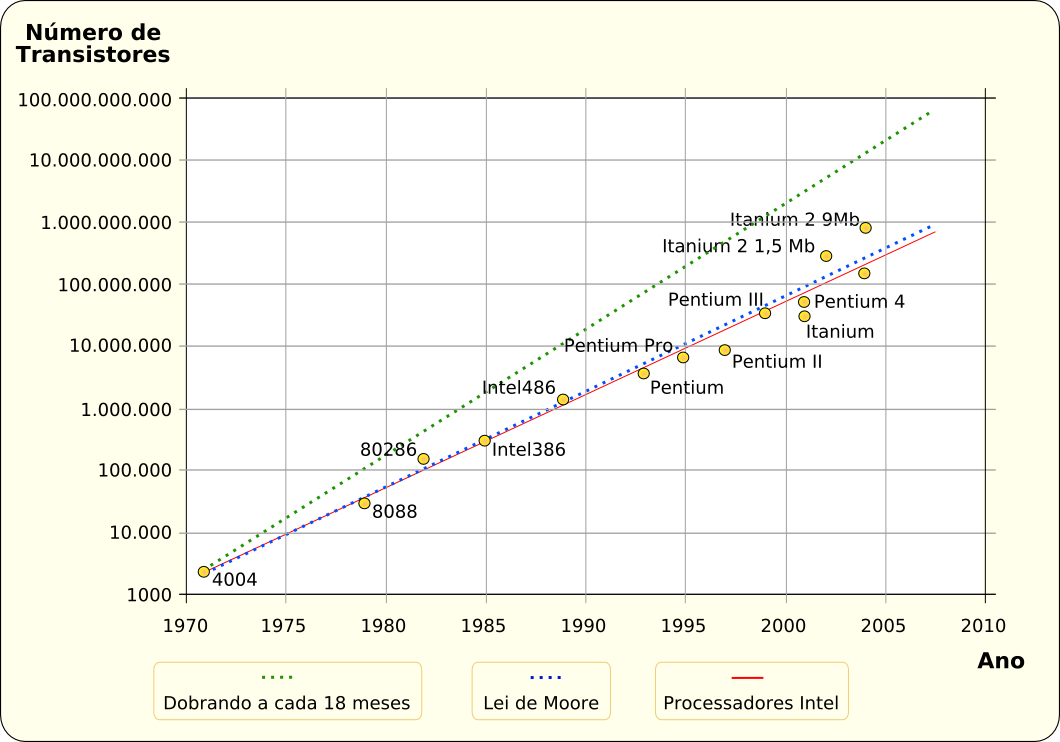
\includegraphics[height=7cm]{Lei_de_moore_2006.png}
  \caption[map]{Lei de Moore \footnote{\tiny
  Fonte: Wikipédia, \url{http://pt.wikipedia.org/wiki/Ficheiro:Lei_de_moore_2006.svg.png},
  em domínio público}}
\end{center}
\end{figure}

%Comentar sobre complexide de algoritmo de escalonamento

\end{frame}

%%%%%%%%%%%%%%%%%%%%%%%%%%%%%%%%%%%%%%%%%%%%%%%%%%%%%%%%%%%%%%%%%%%%%%%%%%%%%%%%
\begin{frame}
\frametitle{}

\begin{figure}[htp]
\begin{center}
  
\includegraphics[height=6cm]{nuvem.png}
\end{center}
\end{figure}

%Comentar sobre complexide de algoritmo de escalonamento

\end{frame}

%%%%%%%%%%%%%%%%%%%%%%%%%%%%%%%%%%%%%%%%%%%%%%%%%%%%%%%%%%%%%%%%%%%%%%%%%%%%%%%%
\begin{frame}
\frametitle{}

\begin{figure}[htp]
\begin{center}
  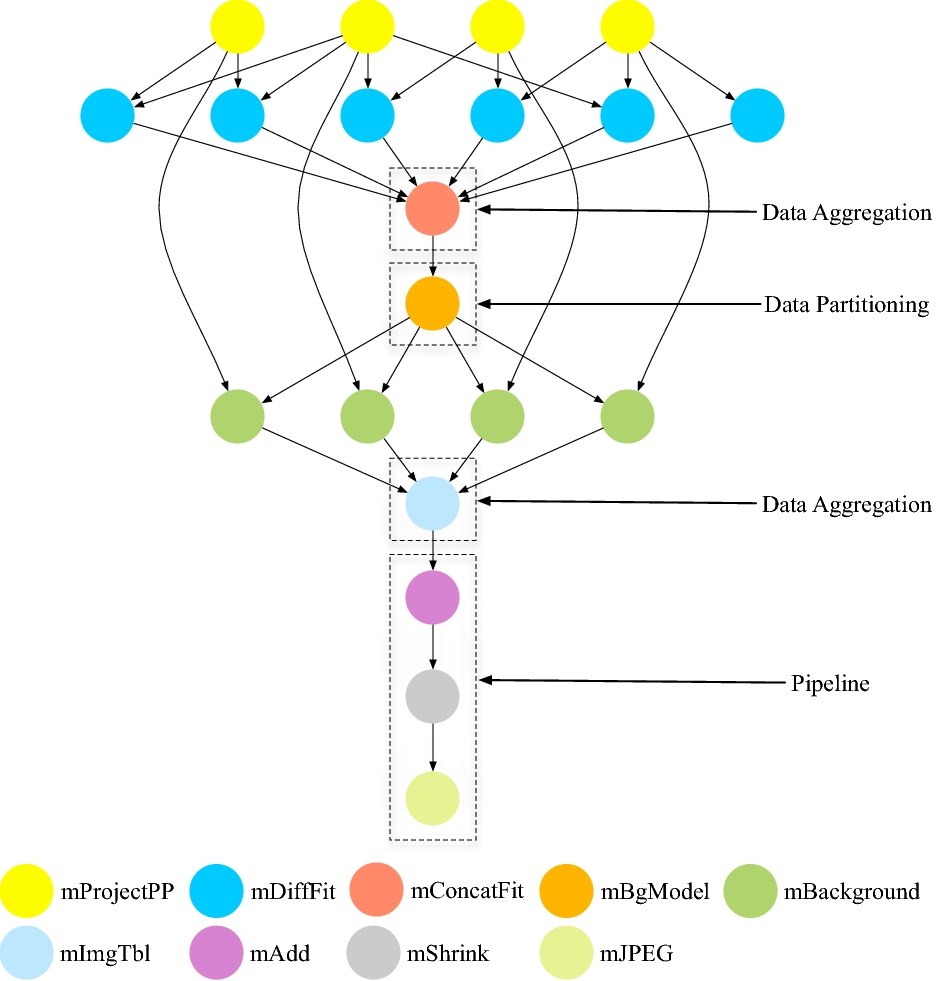
\includegraphics[height=7cm]{Montage.jpg}
  \caption[map]{Montage: Gerador de mosaicos astronômicos \footnote{\tiny
  Fonte: Projeto Pegasus, \url{https://confluence.pegasus.isi.edu/display/pegasus/WorkflowGenerator},
  sob a licença Apache V2}}
\end{center}
\end{figure}

%Comentar sobre complexide de algoritmo de escalonamento

\end{frame}


%%%%%%%%%%%%%%%%%%%%%%%%%%%%%%%%%%%%%%%%%%%%%%%%%%%%%%%%%%%%%%%%%%%%%%%%%%%%%%%%
%%%%%%%%%%%%%%%%%%%%%%%%%%%%%%%%%%%%%%%%%%%%%%%%%%%%%%%%%%%%%%%%%%%%%%%%%%%%%%%%
\section{Conceitos}
\subsection{}

%%%%%%%%%%%%%%%%%%%%%%%%%%%%%%%%%%%%%%%%%%%%%%%%%%%%%%%%%%%%%%%%%%%%%%%%%%%%%%%%
\begin{frame}
\frametitle{Computação em nuvem}
\begin{tikzpicture}
	\pie{1/Monitoramento, 5/Gerenciamento, 18/Equipamentos Elétricos,
                  6/Refrigeração, 18/Instalações, 20/Eletricidade,
                   15/Serviços, 2/Rack, 15/Espaço}

\end{tikzpicture}
\end{frame}

%%%%%%%%%%%%%%%%%%%%%%%%%%%%%%%%%%%%%%%%%%%%%%%%%%%%%%%%%%%%%%%%%%%%%%%%%%%%%%%%
\begin{frame}
\frametitle{Estratégias para economia de energia}
\begin{itemize}
	\item \colorize{n_red}{DVFS}: \emph{Dynamic Voltage and Frequency Scaling}
	\item \colorize{n_blue}{Migração} de máquinas virtuais
	\item \colorize{olive}{Algoritmos de escalonamento} energeticamente eficientes
\end{itemize}
\end{frame}


%%%%%%%%%%%%%%%%%%%%%%%%%%%%%%%%%%%%%%%%%%%%%%%%%%%%%%%%%%%%%%%%%%%%%%%%%%%%%%%%
\begin{frame}
\frametitle{HEFT: \emph{Heterogeneous Earliest Finish Time}}
\begin{itemize}
	\item Publicado em \colorize{n_green}{2002}
	\item Bastante aceito na comunidade científica (Quase \colorize{n_violet}{mil citações})
	\item Duas fases: \colorize{olive}{priorização} e \colorize{RawSienna}{seleção}
\end{itemize}

\end{frame}

%%%%%%%%%%%%%%%%%%%%%%%%%%%%%%%%%%%%%%%%%%%%%%%%%%%%%%%%%%%%%%%%%%%%%%%%%%%%%%%%
\begin{frame}
\frametitle{Fase de priorização}
\begin{itemize}
	\item \colorize{n_red}{Qual} tarefa \colorize{n_red}{escalonar primeiro}?
	\item Algoritmo \colorize{n_green}{offline}
	\item Ordenação topológica:
	
	$$ rank_u(n_i) = \overline{w_i} + \max_{n_j \in succ(n_i)} (\overline{c_{i,j}} + rank_u(n_j)) $$
\end{itemize}
\end{frame}

%%%%%%%%%%%%%%%%%%%%%%%%%%%%%%%%%%%%%%%%%%%%%%%%%%%%%%%%%%%%%%%%%%%%%%%%%%%%%%%%
\begin{frame}
\frametitle{Fase de seleção}
\begin{itemize}
	\item Minimizar o \colorize{n_red}{tempo mais cedo de conclusão} (\emph{Earliest finish time})
	\item Busca por um \colorize{olive}{espaço vago} grande o suficiente
\end{itemize}
\end{frame}


%%%%%%%%%%%%%%%%%%%%%%%%%%%%%%%%%%%%%%%%%%%%%%%%%%%%%%%%%%%%%%%%%%%%%%%%%%%%%%%%
\begin{frame}
%\frametitle{Exemplo}
\begin{columns}[c] % contents are top vertically aligned
	\begin{column}[c]{.6\textwidth} % each column can also be its own environment
		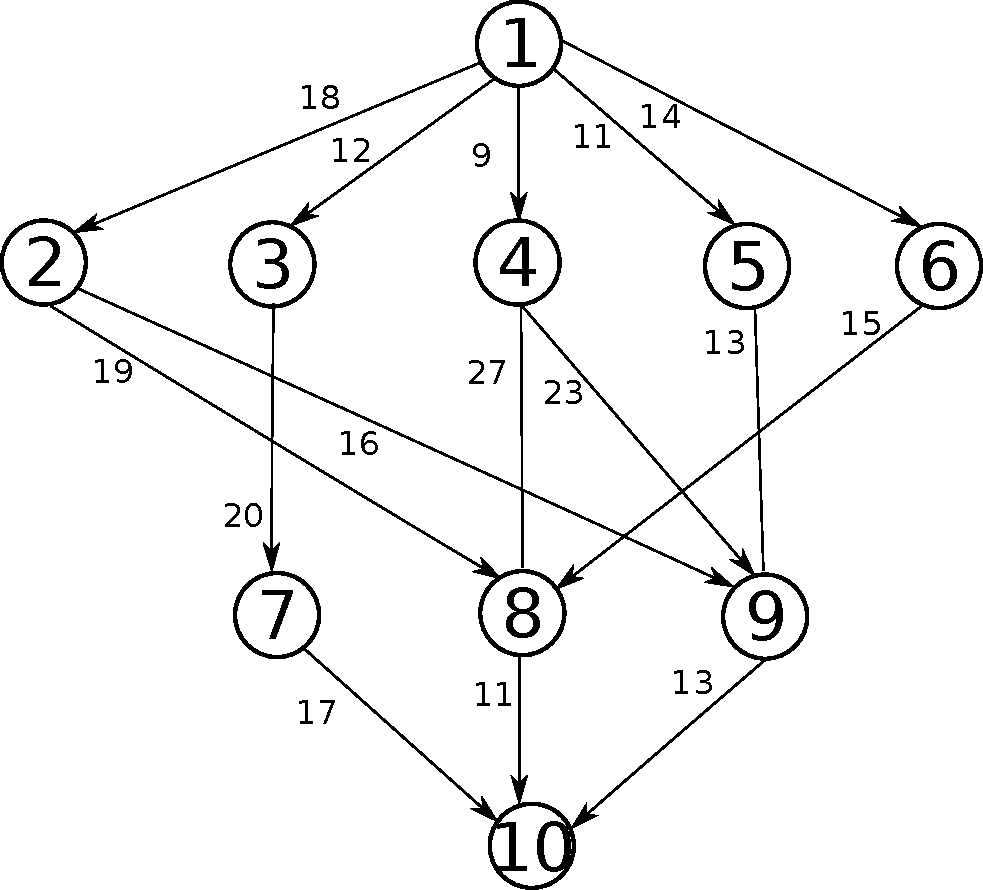
\includegraphics[height=4.5cm]{dag_heft.pdf}
		
		\begin{table}[ht]
		\tiny
		\centering
		\begin{tabular}{|c|c|c|c|c|}
		\hline
		\textbf{Tarefa} & \textbf{P1} & \textbf{P2} & \textbf{P3} & $rank_u(n_i)$ \\ \hline
		1               & 14          & 16          & 9           & 108.000       \\
		2               & 13          & 19          & 18          & 77.000        \\
		3               & 11          & 13          & 19          & 80.000        \\
		4               & 13          & 8           & 17          & 80.000        \\
		5               & 12          & 13          & 10          & 69.000        \\
		6               & 13          & 16          & 9           & 63.333        \\
		7               & 7           & 15          & 11          & 42.667        \\
		8               & 5           & 11          & 14          & 35.667        \\
		9               & 18          & 12          & 20          & 44.333        \\
		10              & 21          & 7           & 16          & 14.667        \\ \hline
		\end{tabular}
		\end{table}
	\end{column}

	\begin{column}[c]{.4\textwidth} % alternative top-align that's better for graphics
		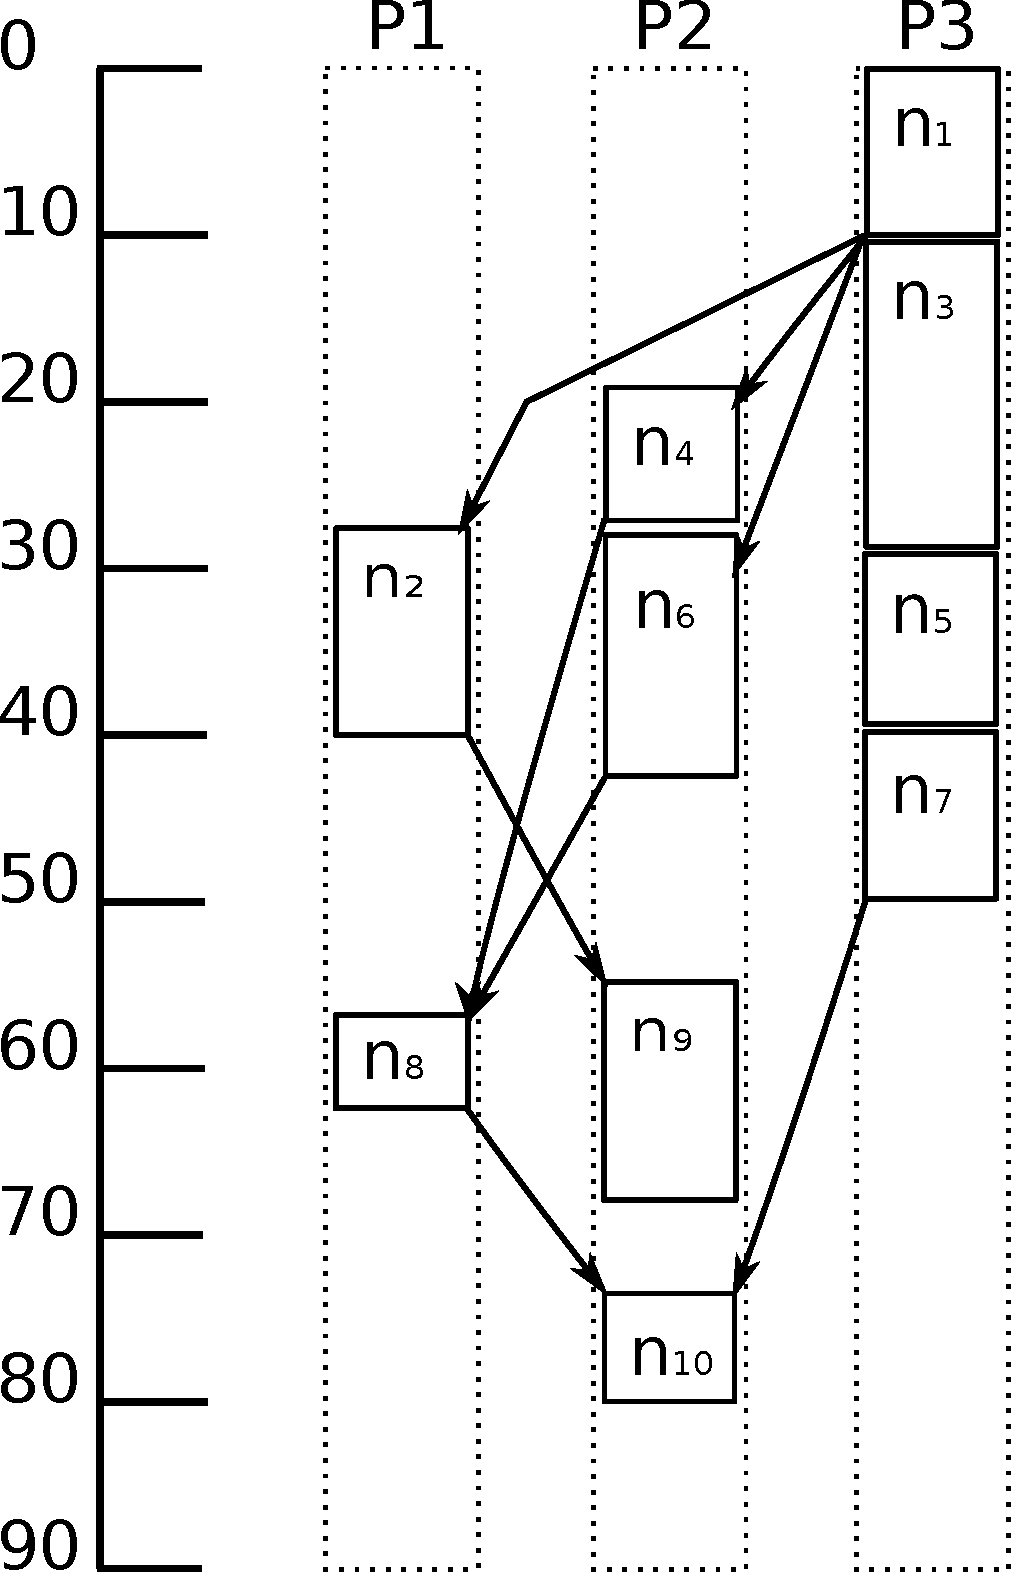
\includegraphics[height=6.5cm]{escalonamento_heft.pdf}
	\end{column}
\end{columns}
\end{frame}



%%%%%%%%%%%%%%%%%%%%%%%%%%%%%%%%%%%%%%%%%%%%%%%%%%%%%%%%%%%%%%%%%%%%%%%%%%%%%%%%
%%%%%%%%%%%%%%%%%%%%%%%%%%%%%%%%%%%%%%%%%%%%%%%%%%%%%%%%%%%%%%%%%%%%%%%%%%%%%%%%
\section{Experimentos}
\subsection{}

%%%%%%%%%%%%%%%%%%%%%%%%%%%%%%%%%%%%%%%%%%%%%%%%%%%%%%%%%%%%%%%%%%%%%%%%%%%%%%%%
\begin{frame}
\frametitle{Simuladores}
\begin{description}
	\item[CloudSim] lançado em \colorize{n_violet}{2010}, já na versão 3, quase 300 citações
	\item[WorkflowSim] lançado em \colorize{n_green}{abril de 2013}
	\item[\textbf{CloudSim\_DVFS}] lançado em \colorize{n_red}{junho de 2013} (!!)
\end{description}

\end{frame}

%%%%%%%%%%%%%%%%%%%%%%%%%%%%%%%%%%%%%%%%%%%%%%%%%%%%%%%%%%%%%%%%%%%%%%%%%%%%%%%%
\begin{frame}
\frametitle{PowerHEFT: Algoritmo proposto}
\begin{itemize}
	\item Variante do HEFT, faz uso de uma estratégia de lookahead
\end{itemize}

\end{frame}


\end{document}

